\documentclass[article,12pt,onesidea,4paper,english,brazil]{abntex2}

\usepackage{lmodern, indentfirst, nomencl, color, graphicx, microtype, lipsum,textcomp}			
\usepackage[T1]{fontenc}		
\usepackage[utf8]{inputenc}		

\setlrmarginsandblock{2cm}{2cm}{*}
\setulmarginsandblock{2cm}{2cm}{*}
\checkandfixthelayout

\setlength{\parindent}{1.3cm}
\setlength{\parskip}{0.2cm}

\SingleSpacing

\begin{document}
	
	\selectlanguage{brazil}
	
	\frenchspacing 
	
	\begin{center}
		\LARGE EFICIÊNCIA DE MÉTODOS DE EXTRAÇÃO DE POTÁSSIO PARA SOLOS DO CONE SUL DE RONDÔNIA\footnote{Trabalho realizado dentro da (área de Conhecimento CNPq/CAPES: Fertilidade do Solo e Adubação) com financiamento do (a) (CNPq/IFRO).}
		
		\normalsize
		Ivanildo Guilherme Henrique\footnote{Bolsista (PIBITI), ivanildo.guilhermee@gmail.com, Campus Colorado do Oeste.} 
		Daniela Souza Silva\footnote{Bolsista (PIBIC), danielaagro22@gmail.com, Campus Colorado do Oeste.} 
		Magno Batista Amorin\footnote{Orientador(a), magno.amorim@ifro.edu.br, Campus Colorado do Oeste.} 
		Fabio Batista de Lima\footnote{Co-orientador(a), fabio.lima@ifro.edu.br, Campus Colorado do Oeste.} 
	\end{center}
	
	% resumo em português
	\begin{resumoumacoluna}
		O estado de Rondônia não possui estudos de calibração, muito menos manuais ou tabelas de recomendação de calagem e adubação. O objetivo deste trabalho foi promover um estudo de correlação para o índice K trocável/extraível em solos do sudoeste amazônico. Foram coletadas amostras de 12 solos representativos, e submetidas a análise química utilizando os extratores Mehlich-1 e NH4Cl 1 mol L-1. Os teores determinados por ambos extratores foram comparados ao determinado pelo método padrão de acetato de amônio 1 mol L-1 a pH 7,0. Todos os extratores testados foram eficientes em determinar a disponibilidade de potássio em solos do sudoeste amazônico, além disso, é possível estabelecer a seguinte ordem decrescente da quantidade média de K extraído: AcNH4> Mehlich-1> NH4Cl.
		
		\vspace{\onelineskip}
		
		\noindent
		\textbf{Palavras-chave}: Acetato de amônio. Cloreto de amônio. K-trocável. 
	\end{resumoumacoluna}
	
	\section*{Introdução}
	
	Estado de Rondônia está localizado na Região da Floresta Amazônia, onde predomina o clima tropical quente e úmido. A maior parte dos solos no Estado de Rondônia originalmente estava coberto pela Floresta Amazônica. Com o passar dos anos e cultivos sucessivos os solos perderam sua fertilidade natural o que reflete diretamente na produção de alimentos do Estado (SCHLINDWEIN et al., 2012).
	Na maioria das propriedades não são adotadas práticas de adubação e calagem e quando feitas as correções são baseadas em manuais de outros estados, o que pode não ser a melhor recomendação. O Estado de Rondônia não possui um manual ou até mesmo uma circular técnica para recomendação de adubação e calagem. Assim, os produtores utilizam manuais de outros estados, o que não é recomendável, uma vez que estes manuais são desenvolvidos para regiões específicas baseados em estudos locais (BARBOZA et al., 2011).
	Nesse sentido, para a utilização racional e mais eficiente destes fertilizantes são necessários estudos de correlação e calibração para cada nutriente, a partir dos quais podem ser geradas tabelas para recomendação de adubação e calagem.
	
	\section*{Material e Método}
	
	O Este estudo foi realizado nas instalações do Laboratório de Análises de Solo, da Faculdade de Agronomia, do Instituto Federal de Rondônia campus Colorado do Oeste. Foram selecionadas amostras de 12 solos representativos de três municípios do cone sul do estado de Rondônia – Colora do Oeste, Cerejeiras e Vilhena – com variabilidade no que se refere as propriedades físicas, químicas e mineralógicas. Todas as amostras foram coletadas a uma profundidade de 0-20 cm de profundidade, destorroadas, secas em estufa a 45°C e tamizadas em peneira com malha de 2 mm de diâmetro, homogeneização da fração < 2 mm, denominada “terra fina seca ao ar” (TFSA) usadas paras as determinações.
	As amostras foram submetidas à análise química de K utilizando as soluções extratoras acetato de amônio 1,0 mol L-1, Mehlich-1 e cloreto de amônio 1,0 mol L-1.
	Paralelamente, dentre as amostras, foram selecionados solos representativos para um estudo a campo. Estes foram incubados em vasos com 5 litros, pH corrigido para 6,0 e 3 repetições.
	Antes do cultivo foi adicionada, em todos os vasos e para todos os solos, uma dose equivalente a 200 kg ha-1 de P2O5 e 200 kg ha-1 de N na forma de Super Fosfato Triplo e Sulfato de Amônia, respectivamente. Para o cálculo da dose, considerou-se o volume de dois milhões de litros de solo por hectare. Após a adição dos fertilizantes, o solo, dentro de cada unidade experimental foi homogeneizado fortemente. Após estes procedimentos, foram semeadas quatro sementes de milho (Zea mayz), cultivar LG 6304 PRO.
	As unidades experimentais foram dispostas em um delineamento inteiramente casualizados, com três repetições, totalizando 36 vasos. O experimento foi conduzido por um período de 30 dias após a emergência, com irrigação diária, mantendo-se a umidade a cerca de 80\% da capacidade de campo. Após esse período, as plantas foram cortadas à altura de um cm do solo.
	A parte aérea das plantas após o cultivo foi coletada e acondicionada em recipientes de papel e deixada em estufa com circulação forçada de ar à temperatura de 65ºC, por 72 horas. Após esse período, estimou-se a massa seca (MS) da parte aérea das plantas de milho, que em seguida foram trituradas em moinho de facas tipo Willey, sendo armazenadas para posterior análise química. O procedimento utilizado para determinação do teor de K da MS foi uma modificação do método descrito na Circular Técnica n° 6 (métodos de análise de tecidos vegetais utilizados na Embrapa solos), por meio da digestão nítrico-perclórica. Sendo o teor de K na solução determinado por espectrofotometria de emissão ótica (ICP-OES).
	A análise dos dados utilizou-se de técnicas de análise de regressão e técnicas de análise de correlação conforme metodologia descrita em Miller e Miller (2005), de modo estabelecer a relação entre o teor de K no solo extraído pelas diferentes soluções e o acumulado pela planta de milho durante o cultivo. Para assim estabelecer a eficiência dos diferentes métodos na estimativa da disponibilidade de K às plantas em solos de munícipios do Cone Sul Estado-RO.
	
	\section*{Resultados e Discussão}
	
	A partir dos valores de coeficiente de correlação, é que se determinou a eficiência de predição dos diferentes métodos, em expressar a disponibilidade de K nos solos amostrados. Os teores de K extraído pelas três soluções (AcNH4, Mehlich- 1 e NH4Cl) em correlação com os absorvidos pelas plantas são mostrados na Figura 01.
	Para o extrator Acetato de Amônio, a correlação entre os teores de K extraídos pela solução e o K extraído da planta é mostrada na figura 1A. O coeficiente de determinação foi de 0,9018.
	A relação entre a quantidade extraída de K pelo método NH4Cl e a absorvida por plantas de milho é apresentadas na figura 1B, sendo o coeficiente de correlação
	(r) 0,8783. A relação entre os teores de K extraídos pela solução de Mehlich-1 e o K acumulado é mostrada na figura 1C. O coeficiente de determinação foi de 0,8269. Os resultados concordam com os obtidos por (MEDEIROS et al., 2010; BORTOLON
	et al, 2010).
	
		\begin{figure}[h]
		\centering
		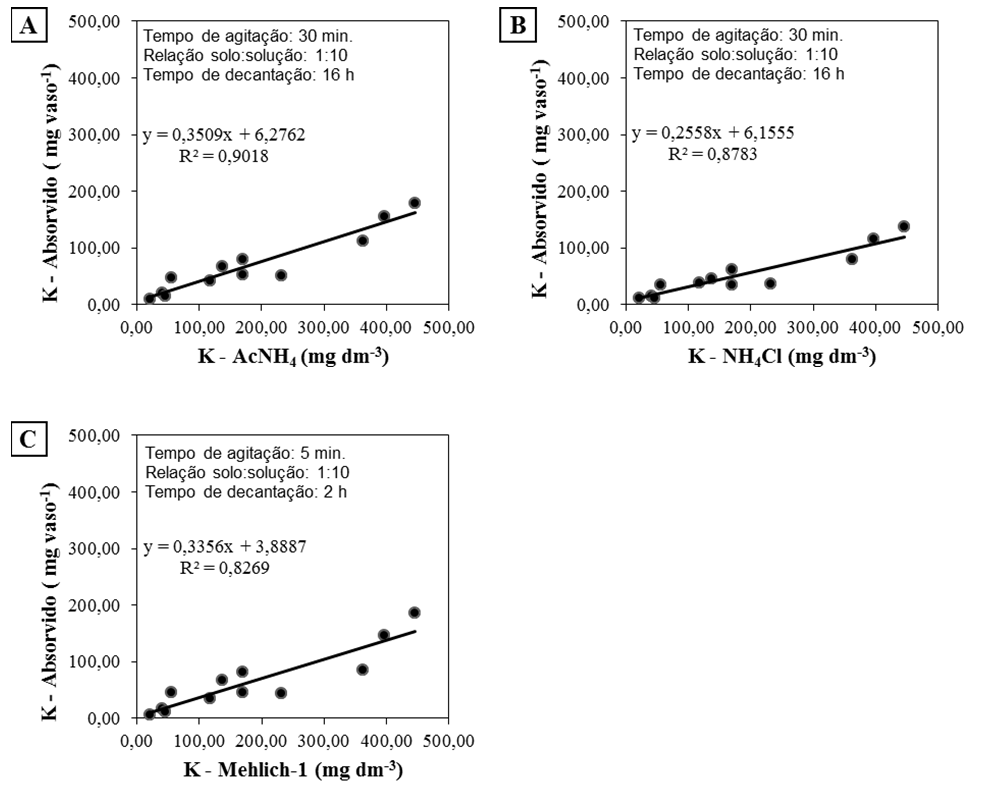
\includegraphics[width=0.7\linewidth]{pip15.png}
		\caption{Relação entre a quantidade de K absorvido por plantas de milho e a extraída dos solos por AcNH4, NH4Cl e M1. IFRO, 2016.}
	\end{figure}
	
	Com tudo, nota-se que todos os métodos foram eficientes na estimativa da disponibilidade de K às plantas em solos de RO. Resultados semelhantes foram obtidos por Kroth (1998), Schlindwein \& Gianello (2005) e Bortolon et al. (2009b) para solos do RS.
	Pois, de maneira geral todos os métodos de extração de K estudados foram altamente correlacionados entre si e apresentaram baixa dispersão de pontos quando comparados dois a dois (figura 01), indicando que os extratores foram eficientes na predição da disponibilidade de K para as plantas, considerando a grande variabilidade mineralógica dos solos utilizados neste estudo.
	
	\section*{Conclusões}
	
	A disponibilidade de potássio para as plantas em solos do sudoeste amazônico pode ser determinada pelos métodos testados no presente trabalho.
	Quando se relaciona os extratores à quantidade de K acumulado por plantas de milho, é possível estabelecer a seguinte ordem decrescente da quantidade média de K extraído do solo nesse trabalho: AcNH4> NH4Cl> Mehlich-1.
	
	\section*{Instituição de Fomento}
	
	Instituto Federal de Educação, Ciências e Tecnologia de Rondônia, Campus
	Colorado do Oeste – IFRO.
	Conselho Nacional de Desenvolvimento Científico e Tecnológico – CNPq.
	
	\section*{Referências}
	
	BARBOZA et al., Fertilidade de Solos em Rondônia. \textbf{Enciclopédia Biosfera}, Centro Científico Conhecer - Goiânia, vol.7, N.13; 2011.
	
	BORTOLON, L.; GIANELLO, C. \& SCHLINDWEIN, J.A. \textbf{disponibilidade de potássio para as plantas em solos do sul do brasil estimada por métodos multielementares}. R. Bras. Ci. Solo, 34:1753-1761, 2010.
	
	BORTOLON, L.; GIANELLO, C. \& SCHLINDWEIN, J.A. Métodos de extração de fósforo e potássio no solo sob sistema plantio direto. \textbf{Ci. Rural}, 39:2400-2407, 2009b.
	
	KROTH, P.L. \textbf{Disponibilidade de fósforo no solo para as plantas e fatores que afetam a extração por resina de troca em membrana.} Porto Alegre, Universidade Federal do Rio Grande do Sul, 1998.168p. (Tese de Mestrado).
	
	MEDEIROS, J. S.; OLIVEIRA, F. H. T.; ARRUDA, J. A.; VIEIRA, M. S.; FONTES, M.
	P. F. Eficiência de extratores de potássio disponível em solos do estado da paraíba com graus de desenvolvimento pedogenético diferentes. \textbf{R. Bras. Ci. Solo}, 34:183- 194, 2010.
	
	MILLER, J.C. \& MILLER, J.N. \textbf{Statistics and chermometrics for analytical chemistry}. 5th ed.Pearson Education Limited, 2005. 268p.
	
	SCHLINDWEIN, J. A. et al. Solos de Rondônia: Usos e perspectivas. \textbf{Revista Brasileira de Ciências da Amazônia}, v1, n1. 2012.
	
	SCHLINDWEIN, J.A. \& GIANELLO, C. Doses de máxima eficiência econômica de fósforo e potássio para as culturas cultivadas no sistema plantio direto. \textbf{R. Plantio Direto}, 85:20-25, 2005
	
\end{document}